\documentclass{source/Report}

\major{地理信息科学}
\name{陈杰伟}
\title{RV64 用户态程序}
\stuid{3200101205}
\college{地球科学学院}
\date{\today}
\lab{玉泉曹光彪-西503}
\course{操作系统}
\instructor{寿黎但}
\grades{}
\expname{RV64 用户态程序}
\exptype{编程实验}
\partner{无}

\begin{document}
\makecover
\makeheader
\section{实验目的}

- 创建用户态进程,并设置 sstatus来完成内核态转换至用户态。

- 正确设置用户进程的用户态栈和内核态栈, 并在异常处理时正确切换。

- 补充异常处理逻辑,完成指定的系统调用( SYS\_WRITE, SYS\_GETPID )功能。

\section{实验环境}
Ubuntu 20.04

\section{实验步骤}
\subsection{创建用户态进程}

由于多个用户态进程需要保证相对隔离,因此不可以共用页表。为每个用户态进程都创建一个页表。修改 task\_struct 如下。

\begin{lstlisting}[language = c, title = {task\_struct}]
    // proc.h 

    typedef unsigned long* pagetable_t;
    
    struct thread_struct {
        uint64_t ra;
        uint64_t sp;                     
        uint64_t s[12];
    
        uint64_t sepc, sstatus, sscratch; 
    };
    
    struct task_struct {
        struct thread_info* thread_info;
        uint64_t state;
        uint64_t counter;
        uint64_t priority;
        uint64_t pid;
    
        struct thread_struct thread;
    
        pagetable_t pgd;
    };
\end{lstlisting}

对 task\_init做如下修改

1.通过 alloc\_page 接口申请一个空的页面来作为 U-Mode Stack

2.为每个用户态进程创建自己的页表 并将 uapp 所在页面,以及 U-Mode Stack 做相应的映射,同时为了避免 U-Mode 和 S-Mode 切换的时候切换页表,将内核页表 ( swapper\_pg\_dir ) 复制到每个进程的页表中

3.用户文件需拷贝至内存(uapp段是在模拟硬盘)

4.对每个用户态进程将 sepc 修改为 USER\_START,配置修改好 sstatus 中的 SPP ( 使得 sret 返回至 U-Mode ), SPIE ( sret 之后开启中断 ), SUM ( S-Mode 可以访问 User 页面 ), sscratch 设置为 U-Mode 的 sp,其值为 USER\_END (即  U-Mode Stack 被放置在 user space 的最后一个页面)。

\begin{lstlisting}[language = c, title = {task\_init}]
    void task_init()
    {
         // idle settings
    
        int i = 0;
        for (i = 1; i < NR_TASKS; ++i)
        {
            task[i] = (struct task_struct *)kalloc();
    
            task[i]->state = TASK_RUNNING;
    
            task[i]->counter = 0;
            task[i]->priority = rand();
    
            task[i]->pid = i;
    
            task[i]->thread.ra = (uint64)&__dummy;
            task[i]->thread.sp = (uint64)task[i] + PGSIZE;
    
            task[i]->pgd = (pagetable_t)alloc_page();
            //用户态页表
            task[i]->pgd = (uint64 *)memcpy(task[i]->pgd, swapper_pg_dir, 512 * sizeof(uint64));
            //复制内核页表到用户页表
    
            create_mapping(task[i]->pgd, (uint64)USER_END - (uint64)PGSIZE, (uint64)alloc_page() - (uint64)PA2VA_OFFSET, (uint64)PGSIZE, (uint64)VM_USER_PERM_R_W_X);
            //对user stack的映射
    
            uint64_t uapp_pg_size = (uint64)(((uint64)uapp_end - (uint64)uapp_start) / (uint64)PGSIZE);
            if ((uint64)uapp_end - (uint64)uapp_start != (uint64)PGSIZE * uapp_pg_size)
                uapp_pg_size++;
    
            task[i]->uapp = alloc_pages(uapp_pg_size);
            task[i]->uapp = (uint64 *)memcpy(task[i]->uapp, (uint64)uapp_start, (uint64)uapp_end - (uint64)uapp_start); //拷贝user space至自己的空间
    
            Elf64_Ehdr *ehdr = (Elf64_Ehdr *)task[i]->uapp;
    
            if (ehdr->e_ident[EI_MAG0] != ELFMAG0 || ehdr->e_ident[EI_MAG1] != ELFMAG1 || ehdr->e_ident[EI_MAG2] != ELFMAG2 || ehdr->e_ident[EI_MAG3] != ELFMAG3)
            {
                task[i]->thread.sepc = (uint64)USER_START;
                task[i]->thread.sscratch = (uint64)USER_END;
                task[i]->thread.sstatus = (uint64)0 + ((uint64)1 << 5) + ((uint64)0 << 8) + ((uint64)1 << 18);
    
                create_mapping(task[i]->pgd, (uint64)USER_START, (uint64)task[i]->uapp - (uint64)PA2VA_OFFSET, (uint64)uapp_end - (uint64)uapp_start, (uint64)VM_USER_PERM_R_W_X);
                //对user space的映射
            }
    
            else
                load_program(task[i]);
        }
    
\end{lstlisting}

注:为拷贝内存方便起见在mm中加入memcpy接口

\begin{lstlisting}[language = c, title = {memcpy}]
    void *memcpy(void *dst, const void *src, uint64 n)
    {
    
        if (dst == NULL || src == NULL || n <= 0)
            return NULL;
    
        char *pdst = (char *)dst;
        char *psrc = (char *)src;
    
        if (pdst > psrc && pdst < psrc + n)
        {
            pdst = pdst + n - 1;
            psrc = psrc + n - 1;
    
            while (n--)
                *pdst-- = *psrc--;
        }
    
        else
        {
            while (n--)
                *pdst++ = *psrc++;
        }
    
        return dst;
    }
\end{lstlisting}

修改\_\_switch\_to ,加入 保存/恢复 sepc,sstatus,sscratch 以及 切换页表的逻辑。在切换了页表之后,通过 fence.i 和 vma.fence 来刷新 TLB 和 ICache。

\begin{lstlisting}[language = bash, title = {\_\_switch\_to}]
    __switch_to:
    # save state to prev process

    # restore state from next process

    #切换页表
    li t0, 0x8000000000000000
    ld t1, 8*22(a1)
    li t2, PA2VA_OFFSET
    sub t1, t1, t2
    srl t1, t1, 12
    add t0, t0, t1

    csrw satp, t0

    # flush tlb
    sfence.vma zero, zero

    # flush icache
    fence.i

    #指针移动
    la t0, current
    sd a1, 0(t0)

    ret
\end{lstlisting}

\subsection{修改中断入口/返回逻辑 (\_trap ) 以及中断处理函数 ( trap\_handler )}

1.修改 \_\_dummy,在 S-Mode -> U->Mode 的时候,交换sp和sscratch的值

\begin{lstlisting}[language = bash, title = {\_\_dummy}]
__dummy:
    #转换到U mode的stack,交换运行栈指针
    csrr t0, sscratch
    csrw sscratch, sp
    add sp, zero, t0

    #la t0, dummy
    #csrw sepc, t0
    sret
\end{lstlisting}

2.修改 \_trap 。同理 在\_trap的首尾我们都需要做类似的操作

\begin{lstlisting}[language = bash, title = { \_trap}]
    _traps:
    sd t0, -8(sp)
    addi sp, sp, -8
    csrr t0, sscratch
    beqz t0, _traps_skip_one
    #转换到U mode的stack,交换运行栈指针
    #栈指针切换,如果是内核线程不需要切换栈指针
    csrw sscratch, sp
    add sp, zero, t0

_traps_skip_one:
    #该段将32个寄存器和spec的值写入栈中,每个寄存器64位,并随时更新栈顶的地址
    
    csrr t0, sscratch
    beqz t0, _traps_skip_two
    #转换到U mode的stack,交换运行栈指针
    #栈指针切换,如果是内核线程不需要切换栈指针
    csrw sscratch, sp
    add sp, zero, t0
    ld t0, 0(sp)
    addi sp, sp, 8

_traps_skip_two:
    sret #一定要用sret返回sepc地址!!!
    }
\end{lstlisting}

添加regs结构体,便于方便地读取中断时寄存器值

trap\_handler中补充处理 SYSCALL 的逻辑。 

\begin{lstlisting}[language = c, title = {trap\_handler}]
    else // exception
    {
        switch (trap_type)
        {
        case 8: // Environment call from U-mode
            switch (regs->a7)
            {
            case SYS_WRITE:
                regs->a0 = sys_write(regs->a0, regs->a1, regs->a2);
                break;
            case SYS_GETPID:
                regs->a0 = sys_getpid();
                break;

            default:
                break;
            }

            regs->sepc += 4; //使sepc返回异常触发的后一条指令
            break;
        default:
            break;
        }
    }
\end{lstlisting}

\subsection{添加系统调用}

sys\_write将用户态传递的字符串打印到屏幕上

\begin{lstlisting}[language = c, title = {sys\_write}]
    uint64_t sys_write(unsigned int fd, const char *buf, size_t count)
    {
        int i = 0;
        uint64 output_count = 0;
    
        for (i = 0; i < count; i++)
        {
            sbi_ecall(fd, 0, (uint64) * (buf + i), 0, 0, 0, 0, 0);
            output_count++;
        }
    
        return output_count;
    }
\end{lstlisting}

sys\_getpid获取当前的pid放入a0中返回

\begin{lstlisting}[language = c, title = {sys\_getpid}]
    uint64_t sys_getpid()
    {
        return (uint64)current->pid;
    }
\end{lstlisting}

系统调用后手动将 sepc + 4

\subsection{修改 head.S 以及 start\_kernel}

在 start\_kernel 中调用 schedule() 

\begin{lstlisting}[language = c, title = {start\_kernel}]
    int start_kernel()
    {
        schedule();
        test(); // DO NOT DELETE !!!
    
        return 0;
    }
\end{lstlisting}

将 head.S 中 enable interrupt sstatus.SIE 逻辑注释

\subsection{添加 ELF 支持}

检测到elf头后,按照分段做虚拟内存映射,并且存储正确的指令地址到sepc

\begin{lstlisting}[language = c, title = {load\_program}]
    void load_program(struct task_struct *task)
    {
        Elf64_Ehdr *ehdr = (Elf64_Ehdr *)task->uapp;
    
        uint64_t phdr_start = (uint64_t)ehdr + ehdr->e_phoff;
        int phdr_cnt = ehdr->e_phnum;
    
        Elf64_Phdr *phdr;
        int load_phdr_cnt = 0;
        for (int i = 0; i < phdr_cnt; i++)
        {
            phdr = (Elf64_Phdr *)(phdr_start + sizeof(Elf64_Phdr) * i);
            if (phdr->p_type == PT_LOAD)
                switch (phdr->p_flags)
                {
                case PF_R:
                    create_mapping(task->pgd, (uint64_t)phdr->p_vaddr, (uint64)ehdr - (uint64)PA2VA_OFFSET + (uint64)phdr->p_offset, (uint64)phdr->p_memsz, VM_USER_PERM_R);
                    break;
                case PF_R + PF_W:
                    create_mapping(task->pgd, (uint64_t)phdr->p_vaddr, (uint64)ehdr - (uint64)PA2VA_OFFSET + (uint64)phdr->p_offset, (uint64)phdr->p_memsz, VM_USER_PERM_R_W);
                    break;
                case PF_R + PF_X:
                    create_mapping(task->pgd, (uint64_t)phdr->p_vaddr, (uint64)ehdr - (uint64)PA2VA_OFFSET + (uint64)phdr->p_offset, (uint64)phdr->p_memsz, VM_USER_PERM_R_X);
                    break;
                case PF_R + PF_W + PF_X:
                    create_mapping(task->pgd, (uint64_t)phdr->p_vaddr, (uint64)ehdr - (uint64)PA2VA_OFFSET + (uint64)phdr->p_offset, (uint64)phdr->p_memsz, VM_USER_PERM_R_W_X);
                    break;
                default:
                    break;
                }
        }
    
        // pc for the user program
        task->thread.sepc = ehdr->e_entry;
        // sstatus bits set
        task->thread.sstatus = (uint64)0 + ((uint64)1 << 5) + ((uint64)0 << 8) + ((uint64)1 << 18);
        // user stack for user program
        task->thread.sscratch = (uint64)USER_END;
    }
\end{lstlisting}

\section{运行结果}

纯二进制和ELF文件都可以正确在其用户态虚拟内存上运行并触发系统调用的中断进行正确系统调用,如图一

\begin{figure}[p]
    \centering
    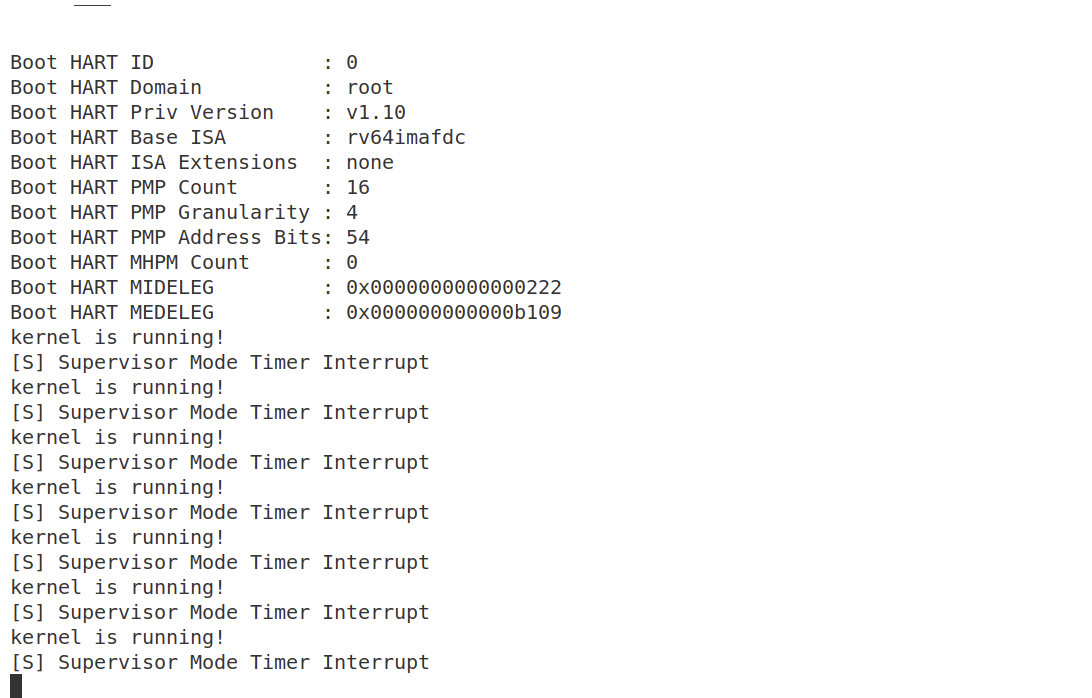
\includegraphics[width = 1\textwidth]{1}
    \caption{结果}
\end{figure}

\section{思考题}

1. 我们在实验中使用的用户态线程和内核态线程的对应关系是怎样的?(一对一,一对多,多对一还是多对多)

   一对一的

2. 为什么 Phdr 中,p\_filesz和 p\_memsz 是不一样大的?

   p\_filesz是segment在文件的字节大小, p\_memsz是 segment在文件的字节大小。

   p\_memsz通常要大于p\_filesz,因为其可能包含存储没有初始化数据的.bss段,将该段数据存储在硬盘中会浪费空间,所以在装入内存后开辟这段空间,导致内存大小和文件大小不同

3. 为什么多个进程的栈虚拟地址可以是相同的?用户有没有常规的方法知道自己栈所在的物理地址?

   因为不同的用户虽然虚拟地址相同但是其所映射的物理地址不同。

   用户没有常规的方法知道自己的栈所在的物理地址,这是虚拟内存的作用之一。



\end{document}

